\chapter{Sequenzdiagramme}
Die folgenden Sequenzdiagramme sollen den Ablauf von einzelnen Anwendungsfällen im PaVoS-System illustrieren. Die Interaktionen der Klassen miteinander in verschiedenen Situationen wird somit verdeutlicht.

\section{Bridge}
In diesem Sequenzdiagramm wird der Ablauf der Bridge beschrieben, die MQTT-Nachrichten in Records umwandelt und diese an Kafka weiterleitet. Die Bridge läuft komplett unabhängig vom restlichen System.\\
Die Bridge kann sich in einer von drei Phasen befinden:
\begin{enumerate}
	\item \textbf{Aufbauphase:} Hier findet die Prüfung der Parameter und das Initialisieren der benötigten Klassen statt.
	\item \textbf{Bereitschaftsphase:} Hier ist die Bridge bereit, Nachrichten von MQTT anzunehmen, zu konvertieren und an Kafka weiter zu senden.
	\item \textbf{Abbauphase:} Hier werden die Verbindungen zu MQTT und Kafka getrennt, anschließend wird die Bridge beendet.
\end{enumerate}
In der Aufbauphase (in diesem Diagramm Operationen 1-5) wird zunächst ein \texttt{JmkbKafkaProducer} erstellt, der intern einen \texttt{KafkaProducer} mit bestimmten Einstellungen initialisiert und eine Verbindung zum Kafka Broker aufbaut. Danach wird ein \texttt{JmkbMqttConsumer} erstellt, der intern einen \texttt{MqttClient} mit bestimmten Einstellungen initialisiert, welcher eine Verbindung zum MQTT-Server aufbaut und die Topics abonniert, die vom FROST-Server angeboten werden.\\\\
Nun beginnt die Bereitschaftsphase. Sobald eine Nachricht beim MqttClient ankommt, wird die Methode \texttt{messageArrived} des \texttt{JmkbMqttConsumer}s aufgerufen. In dieser Methode wird aus der erhaltenen Nachricht die IOT-ID des Sensors gefiltert und die Nachricht wird in das Avro-Format konvertiert. Diese zwei Daten sind dann key und value für das Kafka \texttt{ProducerRecord} und werden über einen Aufruf der \texttt{send}-Methode des \texttt{JmkbKafkaProducer}s in ein solches Format gewandelt. Anschließend wird das Record durch den KafkaProducer an Kafka gesendet.\\\\
In der Abbauphase werden die \texttt{disconnect}-Methoden von \texttt{JmkbMqttConsumer} und \texttt{JmkbKafkaProducer} aufgerufen, die jeweils die Verbindungen zu MQTT und Kafka sauber trennen und die Clients schließen. Die Abbauphase beginnt nur dann, wenn der Nutzer des Programms es willkürlich schließt oder das System es beendet.
\begin{figure}[!hbp]
	\centering
	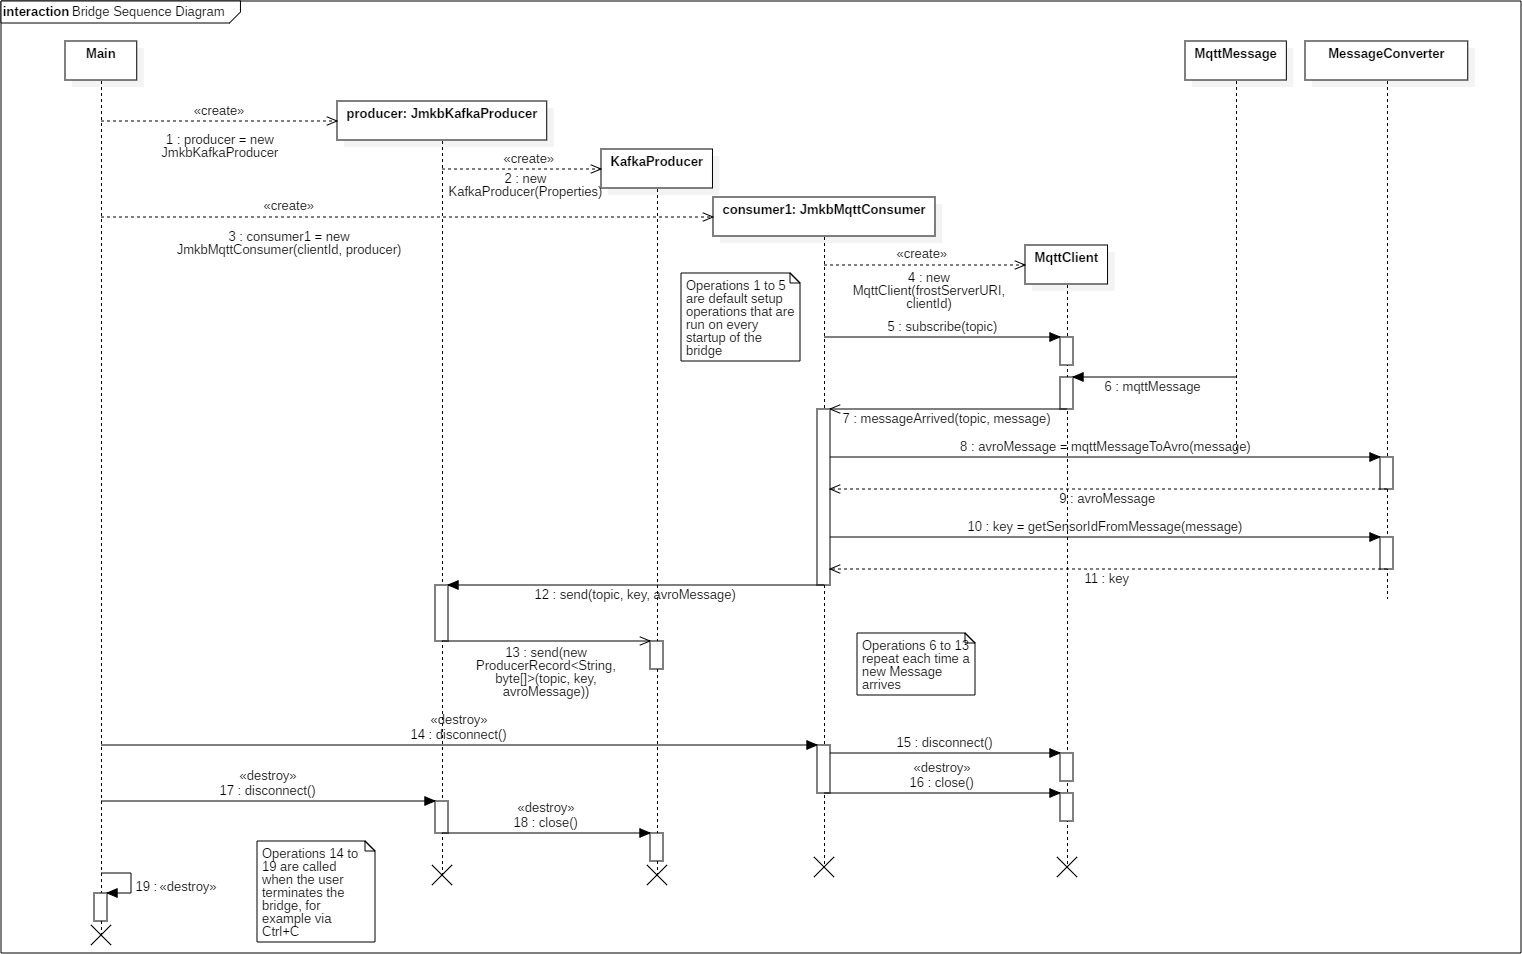
\includegraphics[width=\textheight,angle=90]{images/bridge/BridgeSequenceDiagram.png}
	\caption{Sequenzdiagramm Bridge}
\end{figure}
\newpage

\section{Core}
Beim \texttt{Controller} werden alle Topics, welche von dem MQTT-Producer generierten wurden, in einer Schleife subscribed (abonniert). Dann erzeugt der \texttt{Controller} mit der \texttt{generateOutputtopic} einen neuen Output Topic für eine \texttt{StreamProcessingStrategy}, da dieser ein Output Topic benötigt, um die verarbeiteten Daten abzulagern.
Der \texttt{Controller} konstruiert einen \texttt{TopologyBuilder}, um über diesen die \texttt{StreamProcessingStrategy} ausführen zu können. Mit \texttt{addSource} übergibt der \texttt{Controller} dem \texttt{TopologyBuilder} einen Input Topic, in dem die zu verarbeitenden Daten in einem Kafka Stream enthalten sind.
Der \texttt{Controller} erstellt eine neue \texttt{StreamProcessingStrategy}, die zur Verarbeitung der Inputdaten dienen soll. Der \texttt{Controller} übergibt den \texttt{TopologyBuilder}n mithilfe der \texttt{addProcessor}-Methode diese \texttt{StreamProcessingStrategy}.
Der \texttt{Controller} übergibt den \texttt{TopologyBuilder} mit \texttt{addSink} dem zuvor generierten Output Topic, welcher diesen als Daten-Sink für Daten nutzt, die von der \texttt{StreamProcessingStrategy} verarbeitetet wurden.
Der \texttt{TopologyBuilder} startet nun mit der \texttt{kafkaStreamStart}-Methode die \texttt{StreamProcessingStrategy} und diese beginnt damit durch das Ausführen von \texttt{apply}, aus den Input Topic Daten in den Output Topic zu schreiben, bis der \texttt{TopologyBuilder} \texttt{kafkaStreamClose} aufruft und damit die Verarbeitung stoppt und der \texttt{TopologyBuilder} und die \texttt{StreamProcessingStrategy} zerstört werden.
\begin{figure}[!hbp]
	\centering
	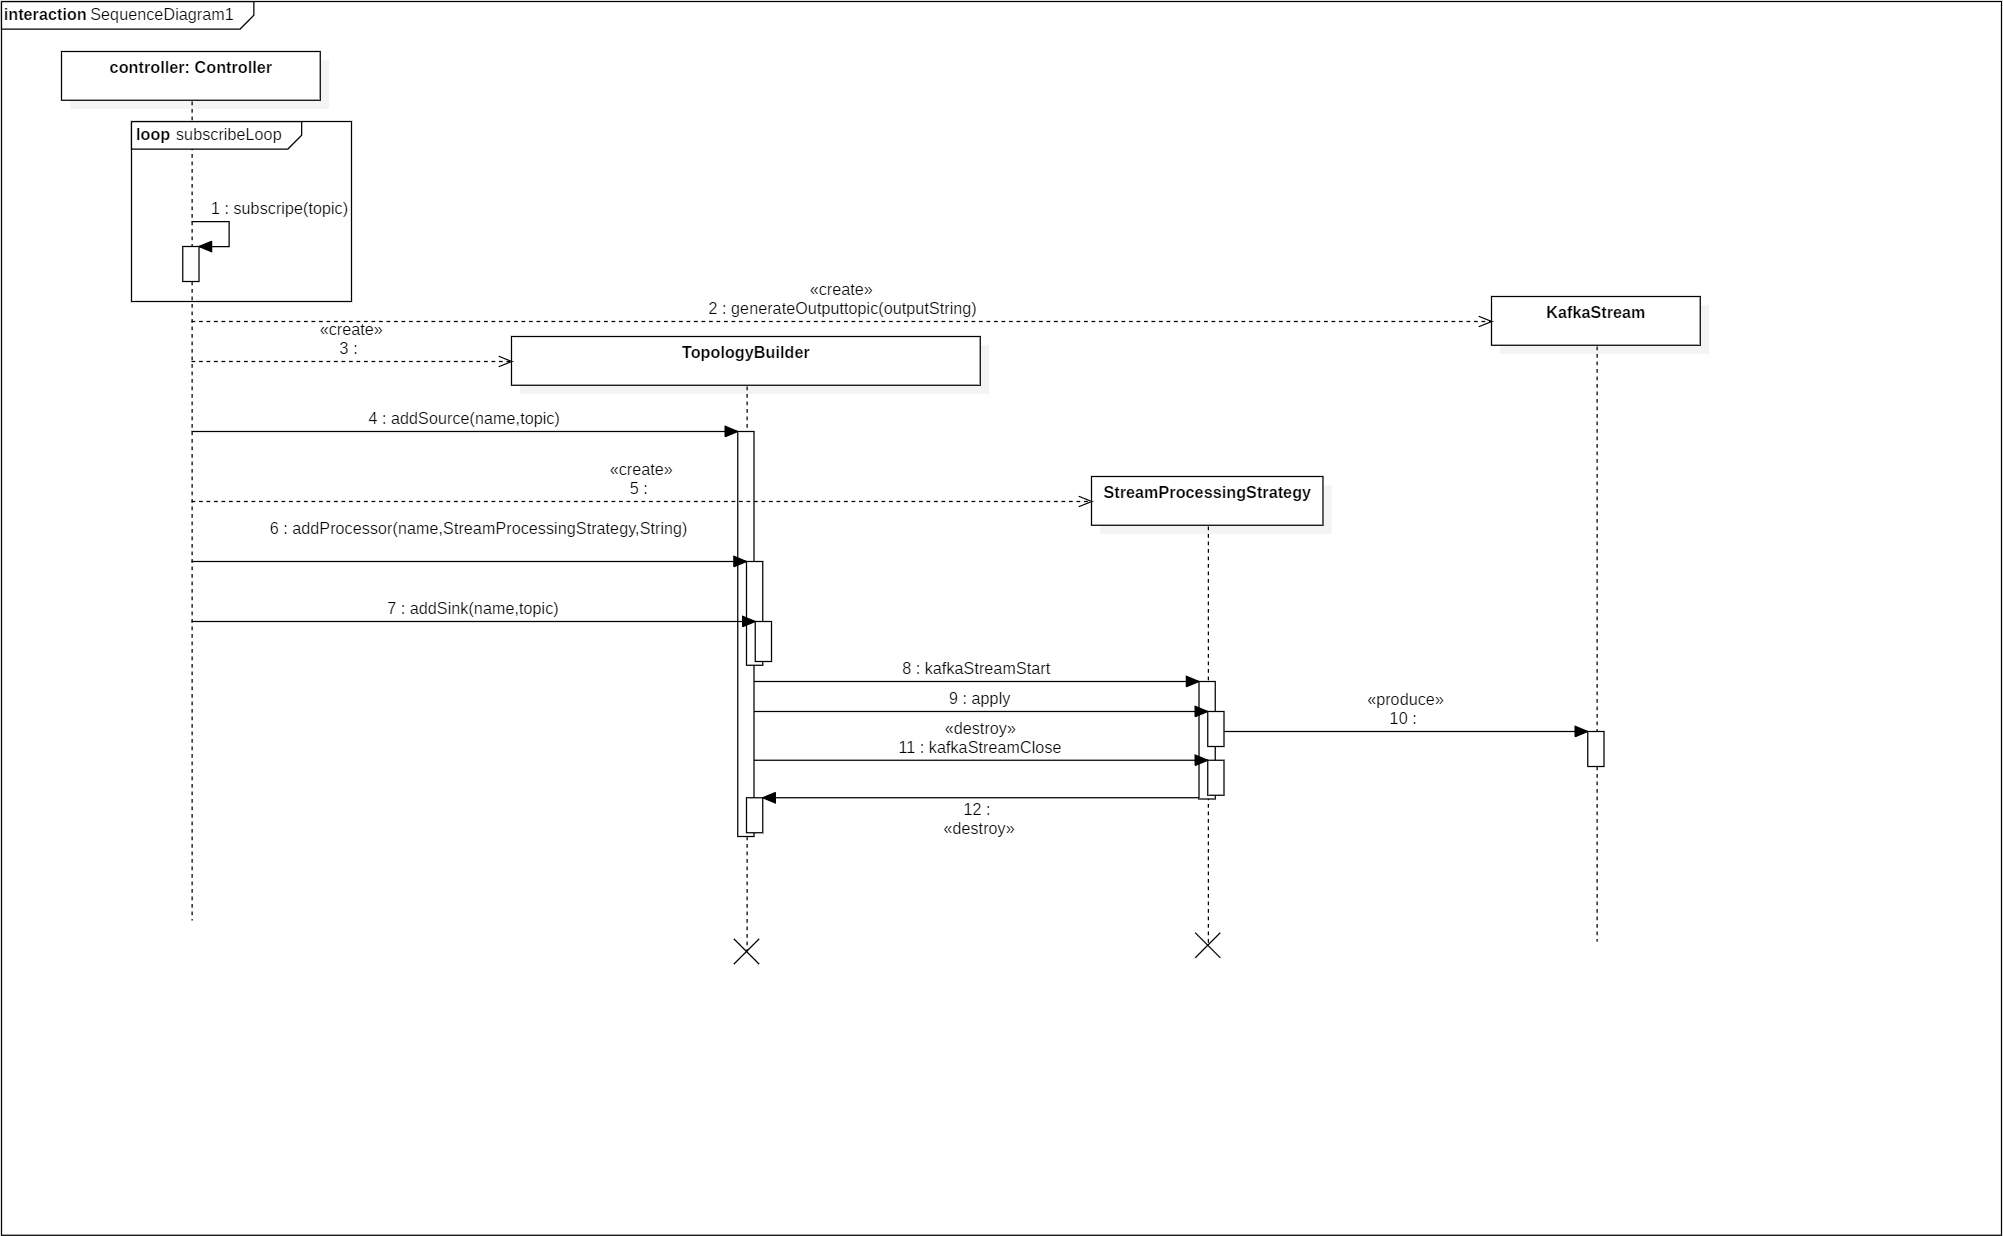
\includegraphics[width=\linewidth]{images/core/CoreSequenceDiagram.png}
	\caption{Sequenzdiagramm Core}
\end{figure}
\newpage

\section{Import}
Bei dem Import wird zuerst in dem Importordner nach Dateien gesucht und danach für jede vorhandene Datei ein separater Importprozess gestartet. Das folgende Sequenzdiagramm stellt diesen Vorgang dar. Hier wird ausschließlich der Import behandelt, wer diesen Anstößt soll nicht Teil des Diagramms sein. \texttt{External} soll hier das Element darstellen, das den Import aufruft. Dazu wird ein \texttt{DataImporter} erstellt und seine Methode \texttt{startImportingFileData} aufgerufen, womit der Importvorgang startet.\\\\
Für jede Datei in dem Importordner wird nun ein \texttt{FrostSender} und ein \texttt{FilePath}, der zum Pfad der Datei passt, erzeugt. Ist dies geschehen wird der \texttt{FileImporter} für diese Datei erschaffen und mit \texttt{addFileData} gestartet. Dazu wird der Pfad und der \texttt{FrostSender} übergeben Aus dem Pfad wird jetzt eine \texttt{FileExtension} generiert, die dazu genutzt wird über den \texttt{ReaderType} eine Instanz einer Implementierung der \texttt{FileReaderStrategy} zu erhalten. Ist die \texttt{FileExtension} nicht bekannt würde es hier zu einer Exception kommen und der Import für diese Datei beendet.\\\\
In diesem Fall wurde als Beispiel eine \texttt{CSVReaderStrategy} genommen. Diese übernimmt den tatsächlichen Import der Daten aus der Datei zum FROST-Server vor. Dazu werden nach und nach einzelne Datensätze aus der Datei ausgelesen und über den \texttt{FrostSender} an den Server gesendet.
\begin{figure}[!hbp]
	\centering
	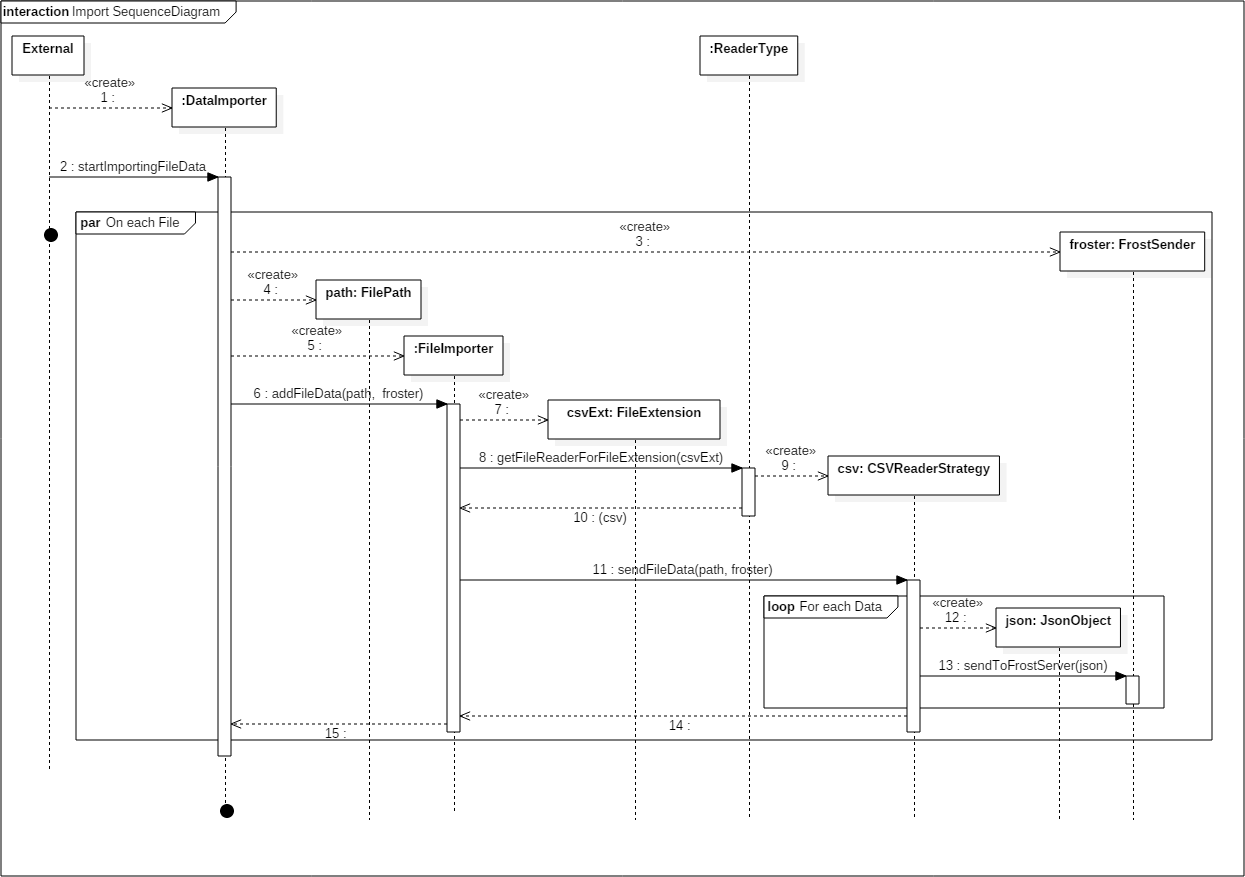
\includegraphics[width=0.9\linewidth]{images/import/ImportSequenceDiagram.png}
	\caption{Sequenzdiagramm Import}
\end{figure}
\newpage

\section{Graphite}
Der Benutzer wählt im Webinterface die Daten aus, die er erhalten will.
Dann erhält das \texttt{Servlet} den Auftrag und leitet dem \texttt{GraphDataTransferController} die Informationen über die Daten weiter, die übertragen werden sollen.
Der \texttt{GraphDataTransferController} erstellt daraufhin einen neuen \texttt{KafkaToGraphiteConsumer}, der ebenfalls diese Informationen erhält und einen \texttt{GraphiteSender} generiert.
Dann wird die Methode \texttt{run} des \texttt{KafkaToGraphiteConsumers} ausgeführt.
Er ruft dann verschiedene Eigenschaften über die \texttt{GraphiteConfig} ab, die benötigt werden um mit Kafka zu kommunizieren.
Weiterhin erzeugt er einen \texttt{KafkaConsumer}, der dann Kafka-Topics abonniert.
Dann prüfen wir ob wir von vorne beginnen wollen.
Danach betreten wir eine Schleife. Hier rufen wir Daten von Kafka ab und speichern sie in einem \texttt{ConsumerRecords} Objekt.
Schlussendlich überprüfen wir, ob die abgerufenen Daten neue Daten enthalten.
Falls ja, senden wir unsere Daten mit Hilfe des \texttt{GraphiteSender}, den wir vorher generiert hatten.
Wenn wir nun die Übertragung der Daten stoppen möchten, müssen wir den \texttt{KafkaConsumer} aufwecken. Dies stoppt die Schleife.
\begin{figure}[!hbp]
	\centering
	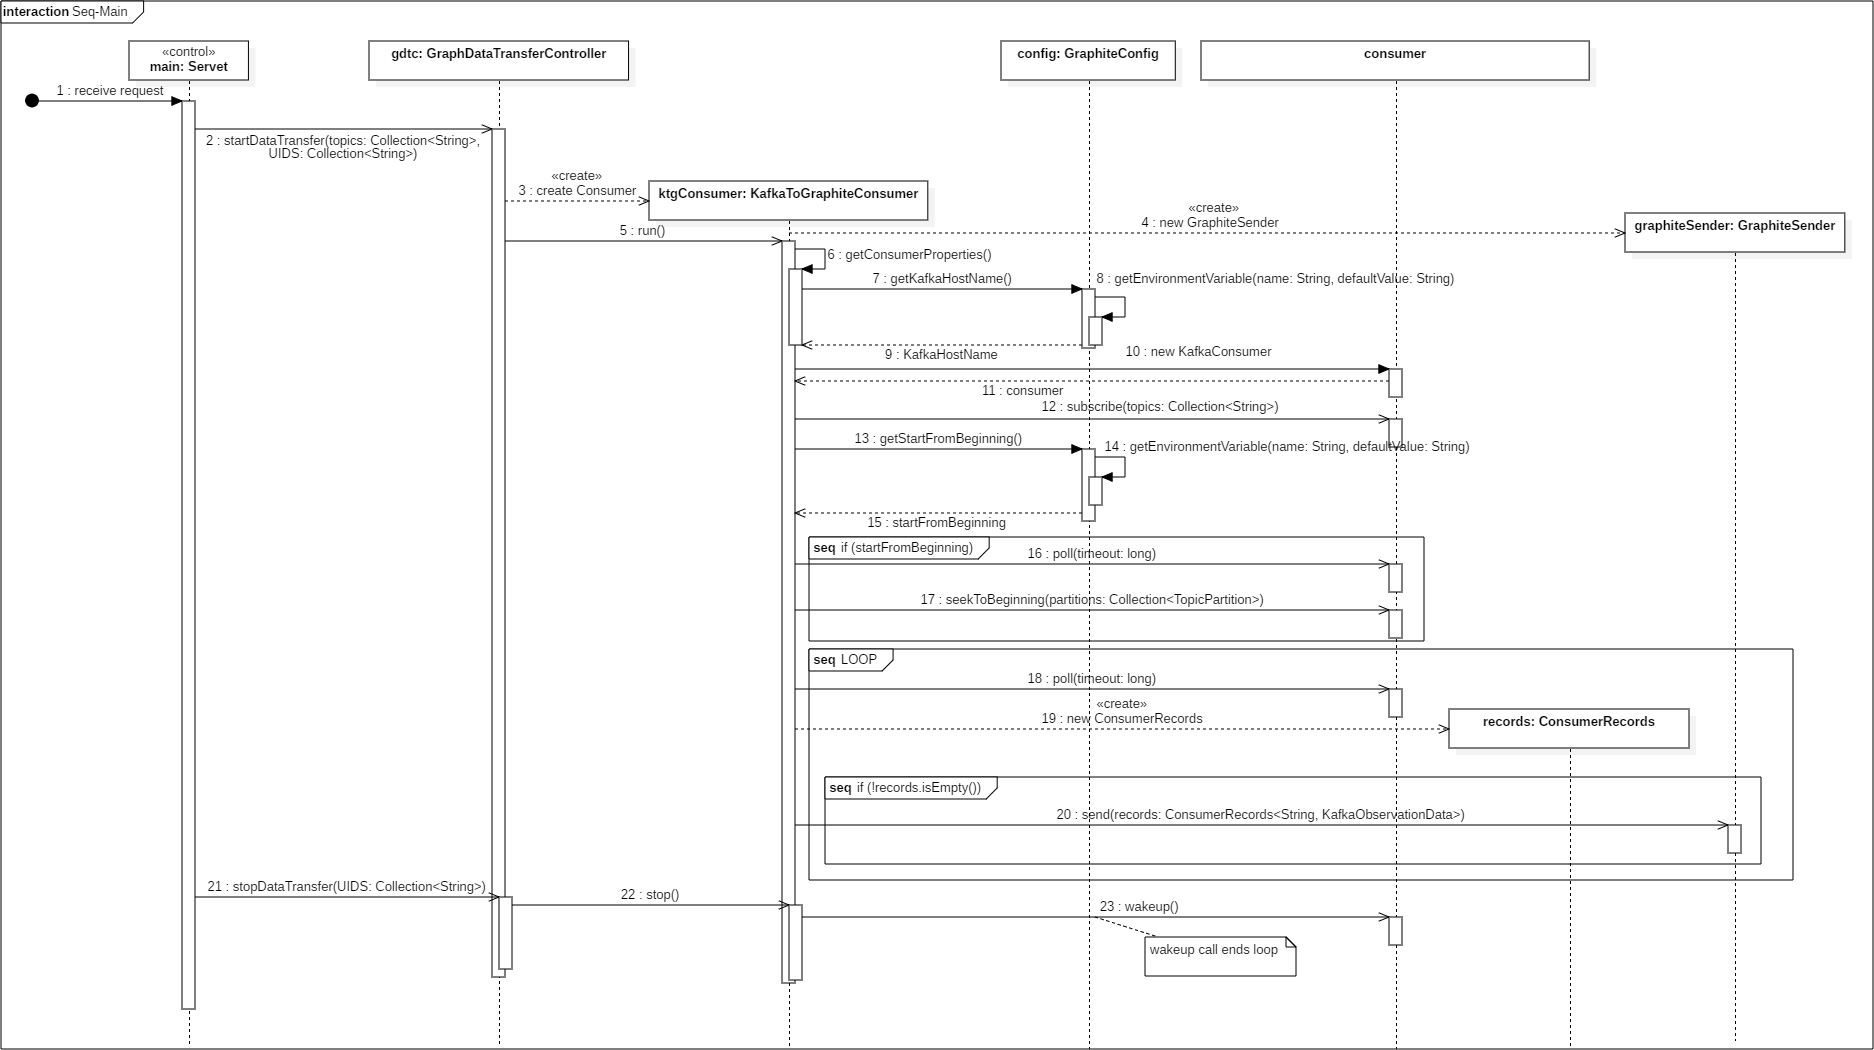
\includegraphics[width=\linewidth]{images/graphite/graphiteMainSequenceDiagram_small.png}
	\caption{Sequenzdiagramm Graphite}
\end{figure}
\newpage
Hier werden die Daten die an Graphite gesendet werden sollen direkt an den \texttt{GraphiteSender} weitergegeben.
Um seine Arbeit zu tun, ruft der \texttt{GraphiteSender} Eigenschaften der \texttt{GraphiteConfig} ab, die notwendig sind, um Daten zu Graphite zu übertragen.
Danach betreten wir die Schleife.
In dieser Schleife, fügt der \texttt{GraphiteSender} jede beobachtete Eigenschaft zur Liste der Daten hinzu, die an Graphite gesendet werden sollen.
Der \texttt{GraphiteSender} tut dies, indem er die Daten zuerst in Metriken konvertiert und dann die Resultate dokumentiert.
Nachdem alle beobachteten Eigenschaften hinzugefügt wurden senden wir die Daten an Graphite.
\begin{figure}[!hbp]
	\centering
	\includegraphics[width=\linewidth]{images/graphite/GraphiteSenderSequenceDiagram.png}
	\caption{Sequenzdiagramm GraphiteSender}
\end{figure}
\newpage

\section{View}
In diesem Funktionsbeispiel der View, wird einem \texttt{MapLayer} einer \texttt{AbstractMap} zunächst ein \texttt{Grid} zugeordnet durch die Methode \texttt{setGrid}. Dann folgt das eigentliche Anzeigen des layers durch die \texttt{displayLayer} Methode. Diese ruft zunächst \texttt{getGrid} um auf die darin enthaltenen \texttt{Cluster} zugreifen zu können durch \texttt{getClusters}. Nun iteriert man über diese und führt für jedes \texttt{Cluster} die Operation \texttt{getTile} aus. Damit hat man Zugriff auf das ihnen zugeordnete \texttt{Tile}. Dies bildet eine graphische Representation und durch die Methode \texttt{display} lässt es sich auf der Karte darstellen. Durch das iterieren über alle \texttt{Cluster} und ihre Visualisierung ergibt sich am ende ein Raster, also die visuelle Representation des \texttt{Grid}.
\begin{figure}[!hbp]
	\centering
	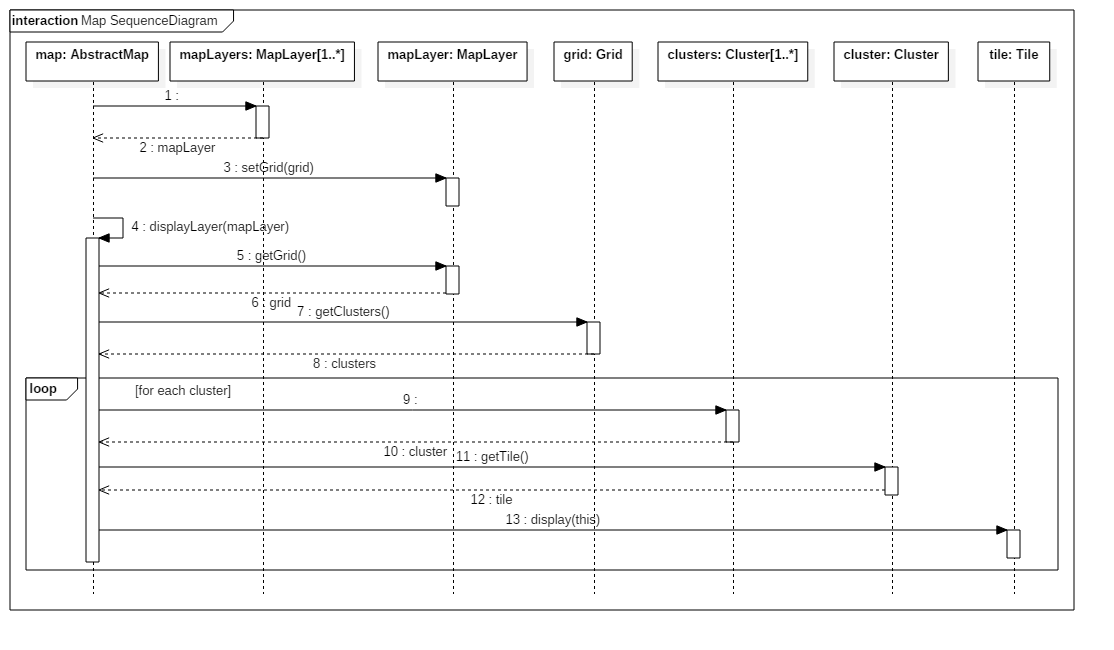
\includegraphics[width=\linewidth]{images/view/ViewSequenceDiagram.png}
	\caption{Sequenzdiagramm View: Anzeigen eines Maplayers}
\end{figure}
\newpage

\section{Export}
Der Export wird in der WebGUI von einem Nutzer angefragt. Die Daten für diesen Export werden an das \texttt{ExportServlet} übertragen, das den tatsächlich Export der Daten in eine Datei verwaltet. Ist diese Datei einmal erstellt, kann diese von dem Nutzer heruntergeladen werden. Dazu mehr in der folgenden Abbildung über den Download. Dieses Sequenzdiagramm zeigt wie der Export der Daten in eine Datei durchgeführt wird.\\\\
Sobald ein Export angestoßen wird, startet das \texttt{ExportServlet} und die Methode \texttt{doGet} wird ausgeführt. Darin werden zuerst die \texttt{ExportProperties} aus der Datei ausgelesen und zu einem Objekt zusammengestellt, das unter anderem eine \texttt{FileExtension} enthält. Danach wird ein \texttt{FileExporter} konstruiert, der in zwei Schritten vorgehen wird, um die Daten zu exportieren.\\\\
Im ersten Schritt, wird durch den Aufruf der \texttt{createFileInformation}-Methode der Export für den späteren Download eindeutig identifiziert, indem ihm eine \texttt{DownloadID} zugewiesen wird. Ein \texttt{AlterableDownloadState} wird erstellt und dessen Methode \texttt{savePersistent} ausgeführt, damit die Information über den Download auch auf dem Server hinterlegt wird, sodass parallel zum Export auch eine Anfrage gesendet werden kann, ob die Datei bereits fertig für den Download ist. Die \texttt{DownloadID} wird dann an den Nutzer zurückgesendet sobald der zweite Teil mit der \texttt{createFile}-Methode des \texttt{FileExporter}s gestartet wurde.\\\\
Im zweiten Schritt, findet dann der tatsächliche Export der Daten in eine Datei statt. Dazu wird zuerst ein \texttt{ExportStreamGenerator} konstruiert, dessen Methode \texttt{createExportStream} einen \texttt{KStream} der gewünschten Daten für den Export erzeugt. Die Gewünschten Daten gehen aus den \texttt{ExportProperties} hervor. Mit der \texttt{FileExtension} aus den \texttt{ExportProperties} kann jetzt ein \texttt{FileType} generiert werden, über dessen Methode \texttt{getFileWriter} eine neue Instanz einer Implementierung einer \texttt{FileWriterStrategy} zurückgegeben wird. Dazu wird die statische Methode \texttt{getFileWriterForFileExtension} der Utilityklasse \texttt{FileTypesUtility} verwendet. In diesem Sequenzdiagramm wird als Beispiel eine Instanz der \texttt{CSVWriterStrategy} verwendet.\\\\
Nun wird ein passender neuer Pfad als \texttt{FilePath} erzeugt, um die Datei zu erzeugen. Zur Erzeugung wird die Methode \texttt{saveToFile} einer Implementierung der \texttt{FileWriterStrategy} genutzt. In diesem Fall einer \texttt{CSVWriterStrategy}. Diese Methode benötigt den Zielpfad und den Stream der Daten und erzeugt daraus eine Datei. Ist dies beendet, wird der \texttt{AlterableDownloadState} dazu genutzt, die nötigen Informationen abzuspeichern. Zuerst wird der Pfad der Datei eingegeben und anschließend wird festgelegt, dass die Datei bereit für den Download ist. Zum Schluss wird noch mit \texttt{savePersistent} sichergestellt, dass andere Instanzen eines \texttt{DownloadState} diese Information abrufen können.
\begin{figure}[!hbp]
	\centering
	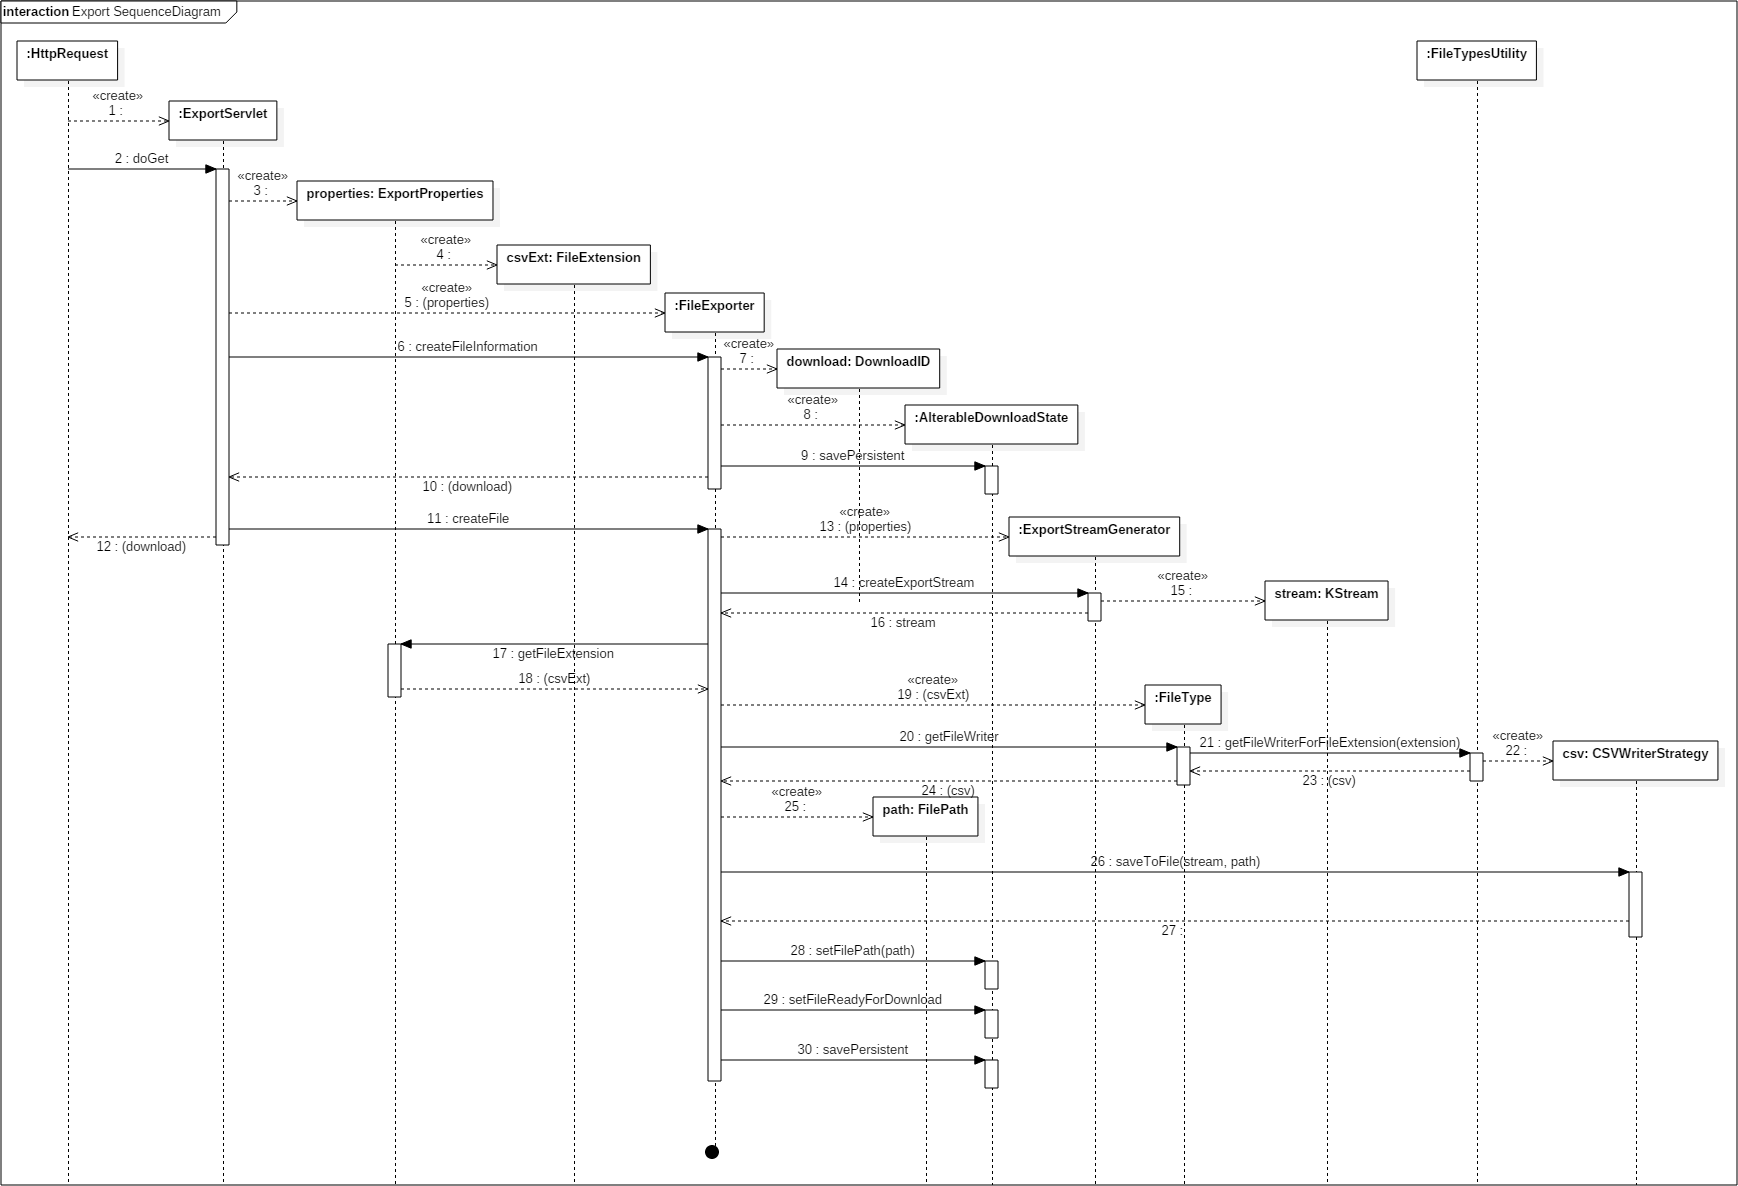
\includegraphics[width=1.25\linewidth,angle=90]{images/export/ExportSequenceDiagram.png}
	\caption{Sequenzdiagramm Export}
\end{figure}
\newpage
Ein Download wird grundsätzlich von einem Nutzer aus einem Browserfenster angefragt. Dazu wird das \texttt{DownloadServlet} benutzt. Diese wird vom Server erstellt sobald eine Anfrage des Nutzer ankommt. Dann wird \texttt{doGet} aufgerufen und das Servlet beginnt mit seiner Aufgabe, die in diesem Sequenzdiagramm dargestellt wird.\\\\
Die Anfrage des Nutzers enthält eine DownloadID, die für eine bestimmte Datei auf dem Server steht. Diese wird benutzt um eine \texttt{DownloadID} Objekt zu erstellen, das dazu dient einen \texttt{DownloadState} zu konstruieren. Dieser holt sich, sobald er erstellt wurde, die Informationen zu dem betreffenden Download. Diese Informationen könnten in einer Datei liegen. Nun wird zuerst geprüft, ob die Datei bereit für den Download ist, dazu dient die Methode \texttt{isFileReadyForDownload}. Ist dies der Fall kann nun mit der \texttt{getFilePath}-Methode nach dem Pfad der Datei gefragt werden. Dieser wird nun vom \texttt{DownloadServlet} genutzt, um die Datei dem Nutzer zu schicken.\\\\
Der Vorgang bei dem \texttt{StatusServlet} ist sehr Ähnlich. Dort geht es darum in Erfahrung zu bringen, ob ein Download bereit ist, um zum Beispiel zu wissen, ob dem Nutzer bereits ein Download-Button gezeigt werden kann. Der einzige Unterschied liegt darin, dass dort nicht nach dem Pfad gesucht wird, sondern gleich das Ergebnis der \texttt{isFileReadyForDownload} zurückgeschickt wird. Aus diesem Grund wurde darauf verzichtet ein separates Sequenzdiagramm dafür zu erstellen.
\begin{figure}[!hbp]
	\centering
	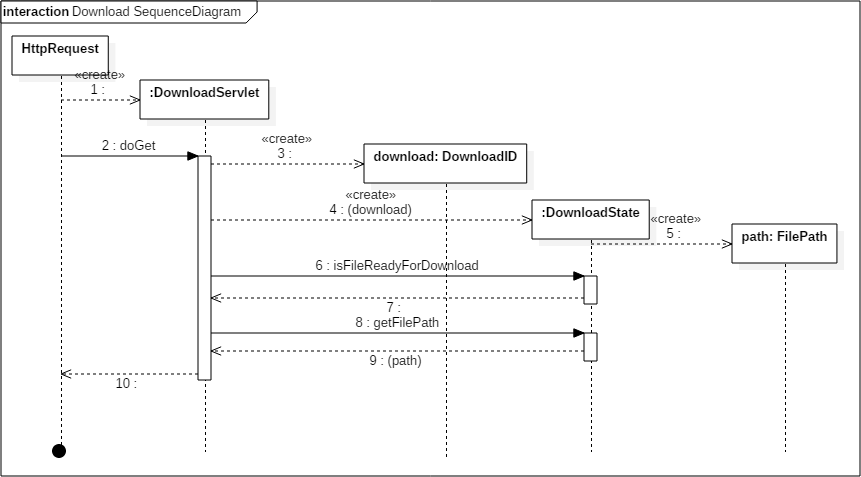
\includegraphics[width=\linewidth]{images/export/DownloadSequenceDiagram.png}
	\caption{Sequenzdiagramm Download}
\end{figure}
